
% 插图环境

\chapter{数值模拟}

\section{模拟$D(s)$和$E(t)$}
设定等距步长 $\delta \in (0,1)$ 及时间区间 $T > 0$.为了在区间 $[0,T]$ 上逼近逆从属过程 $E$,我们遵循 \cite{magdziarz2009stochastic} 中提出的方法.具体来说,首先通过模拟具有独立且平稳增量的从属过程 $D$ 的样本路径来进行逼近.设定 $D_0 = 0$,然后遵循规则 $D_{i\delta} := D_{(i-1)\delta} + Z_i, i=1,2,3,\ldots$,其中 $\{Z_i\}_{i \in \mathbb{N}}$ 为独立同分布的序列,且 $Z_i \stackrel{d}{=} D_{\delta}$.我们在找到整数 $N$ 使得 $T \in [D_N\delta, D_{(N+1)\delta})$ 时停止该过程.请注意,$\mathbb{N}\cup\{0\}$ 值的随机变量 $N$ 确实存在,因为 $D_t \to \infty$ 随着 $t \to \infty$ 几乎必然成立.可以通过下面的算法生成随机变量 $\{Z_i\}$,
\begin{align*}
	Z(i)=\delta^{1/\alpha}\xi_{i}
\end{align*}
其中$\xi_i$是独立同分布的完全偏斜的$\alpha$稳定随机变量,$\xi_i$的实现过程如下:
\begin{align*}
	\xi_i=\frac{\sin(\alpha(V+c_1))}{\left(\cos(V)\right)^{1/\alpha}}\Big(\frac{\cos(V-\alpha(V+c_1))}{W}\Big)^{(1-\alpha)/\alpha}
\end{align*}
其中$c_1 = \frac{\pi}{2}$,随机变量$V$是$(-\frac{\pi}{2},\frac{\pi}{2})$上的均匀分布,$W$是均值为$1$的指数分布.
然后,令
$$
E_t^\delta := \left(\min\{n \in \mathbb{N}; D_{n\delta} > t\} - 1\right)\delta, \quad t \in [0, T].
$$
过程 $E^\delta = (E_t^\delta)_{t \geq 0}$ 的样本路径是具有恒定跳跃大小 $\delta$ 的单调递增阶梯函数,第 $i$ 个等待时间为 $Z_i = D_{i\delta} - D_{(i-1)\delta}$.过程 $E^\delta$ 有效地逼近 $E$;实际上,几乎必然地,
$$
E_t - \delta \leq E_t^\delta \leq E_t \quad \text{对于所有} \quad t \in [0, T].
$$

在\cite{jin2019strong}中对$\Delta E$的处理时,t每次跳$D_{n\delta} - D_{(n-1)\delta}$,于是$E$每次对应改变$\delta$.然而,在我们的离散格式中,选择对t做等距离散,让t每次跳跃的长度是固定的长度h,于是$E$在第i次跳跃对应的变化就是$E_{ih} - E_{(i-1)h}$,这样的离散会导致出现$\Delta E=0$,这是得到收敛阶是$\alpha$的关键.

\section{时间变换的布朗运动驱动的CIR过程}\label{TCCIR}
回忆时间变换的CIR过程
\begin{equation}\label{CIR}
	dy(t)=\kappa(\theta-y(t))dE(t)+\sigma\sqrt{y(t)}dB(E(t)),\quad t\geq0,\quad y(0)>0.
\end{equation}
如果 $2\kappa\theta\geq\sigma^{2}$, 那么 $D=(0,\infty)$ 并且\cref{assum1} 在 $(\alpha,\beta)=$
$(0,\infty)$是成立的. 
另外, 使用It\^{o}公式$X(t)=F((y(t))$,其中$F$是由\cref{Lamperti}定义,即对时间变换的CIR过程进行Lamperti变换可以得到
\begin{equation}
	dX(t)=f(X(t))dE(t)+\frac12\sigma dB(E(t)),\quad t\geq0,\quad X(0)=\sqrt{y(0)}
\end{equation}
其中
\begin{equation}
	f(X)=\dfrac{1}{2}\kappa\left(\theta_vX^{-1}-X\right),\quad X>0
\end{equation}
其中 $\theta_v=\theta-\frac{\sigma^2}{4\kappa}$ ,并且 BEM数值格式如下
\begin{equation}
	X_{t_{i+1}}=X_{t_{i}}+f(X_{t_{i+1}})\Delta E_i+\frac{1}{2}\sigma\Delta B_{E_i},\quad k=0,1,\dots 
\end{equation}
观察到
\begin{equation}
	f'(X)=-\frac{1}{2}\kappa(\theta_vX^{-2}+1)
\end{equation}
以及
\begin{equation}
	f(X)f'(X)+\frac{\sigma^2}{2}f''(X)=-\frac{\kappa^2}{4}(\theta_v^2X^{-3}-X)+\frac{1}{2}\kappa\theta_vX^{-3}\sigma^2.
\end{equation}
因此为了满足\cref{assum3},只需要满足
\begin{equation}
	\sup_{0\leq t\leq T}\mathbb{E}[X(t)^{-3}]=\sup_{0\leq t\leq T}\mathbb{E}[y(t)^{-\frac{3}{2}}] < \infty.
\end{equation}
对于时间变换的CIR过程y(t)的矩有界,即
\begin{equation}
	\sup\limits_{0\leq t\leq T}\mathbb{E}[y(t)^q]<\infty\quad\mathrm{for}\quad q>-\frac{2k\theta}{\sigma^2},
\end{equation}
下面验证,对于由时间变换的的布朗运动驱动的CIR过程\cref{CIR}的精确解矩有界.
\begin{proposition}
	对于由时间变换的布朗运动驱动的CIR过程\cref{CIR},其中$y_0>0$,$1<p<\frac{2K\theta}{\sigma^2}-1$,都存在一个常数C使得
	\begin{equation*}
		\sup\limits_{t\in[0,T]}\mathbb{E}\left[\left(y(t)\right)^{-p}\right]\leq C(1+y(0)^{-p})
	\end{equation*}
\end{proposition}
\begin{proof}
	定义停时$\tau_{n}=\mathrm{inf}\{0<s\leq T;y(s)\leq1/n\}$,通过It\^{o}公式,我们可以得到
	$$\begin{aligned}
		\mathbb{E}_B\left[(y(t\wedge\tau_{n}))^{-p}\right] &=y(0)^{-p}-p\mathbb{E}_B\left[\int_{0}^{t\wedge\tau_{n}}\frac{K(\theta-y(s))}{(y(s))^{p+1}}dE(s)\right]\\
		&+p(p+1)\frac{\sigma^{2}}{2}\mathbb{E}_B\left[\int_{0}^{t\wedge\tau_{n}}\frac{1}{(y(s))^{p+1}}dE(s)\right] \\
		&\leq y(0)^{-p}+pK\int_{0}^{t}\mathbb{E}_B\left(\frac{1}{(y(s\wedge\tau_{n}))^{p}}
		\right)dE(s) \\
		&+\mathbb{E}_B\left[\int_0^{t\wedge\tau_n}\frac{p\left(\frac{(p+1)\sigma^2}{2}-K\theta\right)}{(y(s))^{p+1}}dE(s)\right]
	\end{aligned}$$
	通过计算可以找到正数$\underline C$使得, 当$\frac{(p+1)\sigma^2}{2}-K\theta<0$时,对于任意的 $y(0)=x>0$,都有
	$$\frac{p\left(\frac{(p+1)\sigma^2}{2}-K\theta\right)}{x^{p+1}}\leq \underline C$$
	因此
	$$\mathbb{E}_B\left[(y(t\wedge\tau_n))^{-p}\right]\leq y(0)^{-p}+\underline{C}E(T)+pK\int_0^t\sup_{r\in[0,s]}\mathbb{E}_B\left[(y(r\wedge\tau_n))^{-p}\right]dE(s)$$
	于是由Gronwall不等式,可以得到
	$$\sup\limits_{t\in[0,T]}\mathbb{E}_B\left[(y(t\wedge\tau_n)^x)^{-p}\right]\leq\left(y(0)^{-p}+\underline{C}E(T)\right)\exp(pKE(T))$$
	两边同时取$\mathbb{E}_D$并使用Cauchy-Schwarz不等式,得到
	$$\begin{aligned}
		\sup\limits_{t\in[0,T]}\mathbb{E}\left[(y(t\wedge\tau_n)^x)^{-p}\right]&\leq\mathbb{E}\left[\left(y(0)^{-p}+\underline{C}E(T)\right)\exp(pKE(T))\right]\\
		&\leq\sqrt{\mathbb{E}\left[\left(y(0)^{-p}+\underline{C}E(T)\right)^2\right]\mathbb{E}\left[\exp(2pKE(T))\right]}
	\end{aligned}$$
	从\cite{jum2014strong}可以得到
	\begin{equation}
		\mathbb{E}[E^n(t)]=\frac{n!}{\Gamma(n\alpha+1)}t^{n\alpha}
	\end{equation}
	\begin{equation}
		\mathbb{E}[e^{\lambda E(t)}]<\infty
	\end{equation}
	其中$\lambda \in \mathbb{R},t>0$.最后,让 $n\to+\infty$,我们完成了这个证明.
\end{proof}
\begin{remark}
	在这里只是证明了当$1<p<\frac{2K\theta}{\sigma^2}-1$的时候,矩的存在性,实际上更可以证明$p<\frac{2K\theta}{\sigma^2}$,但是证明起来过于复杂,这里就不在说明,对于我们的结果已经够用了.
\end{remark}
对于\cref{assum3},可以验证只需要保证$1 < \frac{4}{3}\frac{k\theta}{\sigma^2}$成立即可,而这个区间可以被$1<p<\frac{2K\theta}{\sigma^2}-1$包含在内,因此只需要保证p在后者这个区间即可.至于\cref{assum2},在$(0,\infty)$中很容易可以验证存在这样的$\kappa$使之成立.因此由\cref{main th}可以得到,对于时间变换的CIR过程,使用BEM数值格式的强收敛阶是$\alpha$
\section{数值实验}
在我们的数值实验中,我们关注端点$T = 1$处的$L_1$误差,因此我们令
\begin{align*}
	e_T^{i}=\mathbb{E}\left|X_T^{\delta _{15}}-X_T^{\delta _i}\right|
\end{align*}
其中$X_T^{\delta _i}$是步长为$\delta _i$时T处的模拟值,$\delta _i = 2^{-i}$,对于我们的数值实验,取$\theta=0.125,\kappa=2$以及$\sigma=0.5$,采用蒙德卡洛方法,
\begin{align*}
	e_{T}^i\approx\frac{1}{10^3}\sum_{j=1}^{10^3}\left|X_T^{\delta _{15}}-X_T^{\delta _i}\right|.
\end{align*}
选择步长为$2^{-15}$作为参考,通过${2^{-11},2^{-10},2^{-9},2^{-8}}$的步长来估计$L_1$误差.
\section{时间变换的布朗运动驱动的CEV过程}
另外一个比较常用的金融模型是CEV模型,下面是由时变布朗运动驱动的CEV模型
\begin{equation}\label{CEV}
	dy(t)=\kappa(\theta-y(t))dE(t)+\sigma y(t)^\alpha dB_{E(t)}
\end{equation}
其中 $0.5<\alpha<1,\kappa,\theta,\sigma>0.$ 通过变换$X(t)=F(y(t))$的变换之后,其中$F$是由\cref{Lamperti}定义,我们可以得到\cref{assum2}在$(\alpha,\beta)=(0,\infty)$下,是成立的,此时	$$dX(t)=f(X(t))dE(t)+(1-\alpha)\sigma dB(E(t))$$
其中
$$f(X)=(1-\alpha)\left(\kappa\theta X^{-\frac\alpha{1-\alpha}}-\kappa X-\frac{\alpha\sigma^2}2X^{-1}\right),\quad X>0.$$
同时我们需要验证另一个\cref{assum3}.因为 $\alpha>0.5$, 于是$\frac{1}{1-\alpha}>2$,因此
$$f^{\prime}(X)=-\alpha\kappa\theta X^{-\frac1{1-\alpha}}-(1-\alpha)\kappa+(1-\alpha)\frac{\alpha\sigma^2}2X^{-2},\quad X>0$$
同时我们又有
$$f^{\prime\prime}(X)=\frac\alpha{1-\alpha}\kappa\theta X^{-\frac{2-\alpha}{1-\alpha}}-(1-\alpha)\alpha\sigma^2X^{-3}.$$
下面验证,对于由时间变换的的布朗运动驱动的CEV过程\cref{CEV}的精确解矩有界.
\begin{proposition}
	对于由时间变换的布朗运动驱动的CEV过程\cref{CEV},其中$X_0>0$,对于任意的$\frac{1}{2}<\alpha<1$和任意的$p>0$,都存在一个常数C使得
	\begin{equation*}
		\sup\limits_{t\in[0,T]}\mathbb{E}\left[\left(y(t)\right)^{-p}\right]\leq C(1+y(0)^{-p})
	\end{equation*}
\end{proposition}
\begin{proof}
	定义停时$\tau_{n}=\mathrm{inf}\{0<s\leq T;y(s)\leq1/n\}$,通过It\^{o}公式,我们可以得到
	$$\begin{aligned}
		\mathbb{E}_B\left[(y(t\wedge\tau_{n}))^{-p}\right] &=y(0)^{-p}-p\mathbb{E}_B\left[\int_{0}^{t\wedge\tau_{n}}\frac{K(\theta-y(s))}{(y(s))^{p+1}}dE(s)\right]\\
		&+p(p+1)\frac{\sigma^{2}}{2}\mathbb{E}_B\left[\int_{0}^{t\wedge\tau_{n}}\frac{1}{(y(s))^{p+2(1-\alpha)}}dE(s)\right] \\
		&\leq y(0)^{-p}+pK\int_{0}^{t}\mathbb{E}_B\left(\frac{1}{(y(s\wedge\tau_{n}))^{p}}
		\right)dE(s) \\
		&+\mathbb{E}_B\left[\int_0^{t\wedge\tau_n}\left(p(p+1)\frac{\sigma^2}{2}\frac{1}{(y(s))^{p+2(1-\alpha)}}-p\frac{K\theta}{(y(s))^{p+1}}\right)dE(s)\right]
	\end{aligned}$$
	可以找到正数$C$使得, 对于任意的 $y(0)=x>0$,都有
	$$\left(p(p+1)\frac{\sigma^2}{2}\frac{1}{x^{p+2(1-\alpha)}}-p\frac{K\theta}{x^{p+1}}\right)\leq C$$
	通过计算可以得到,$\underline C=p(2\alpha-1)\frac{\sigma^2}{2}\left[(p+2(1-\alpha))\frac{\sigma^2}{2K\theta}\right]^{\frac{p+2(1-\alpha)}{2\alpha-1}}$ 是最小的上界. 因此
	$$\mathbb{E}_B\left[(y(t\wedge\tau_n))^{-p}\right]\leq y(0)^{-p}+\underline{C}E(T)+pK\int_0^t\sup_{r\in[0,s]}\mathbb{E}_B\left[(y(r\wedge\tau_n))^{-p}\right]dE(s)$$
	于是由Gronwall不等式,可以得到
	$$\sup\limits_{t\in[0,T]}\mathbb{E}_B\left[(y(t\wedge\tau_n)^x)^{-p}\right]\leq\left(y(0)^{-p}+\underline{C}E(T)\right)\exp(pKE(T))$$
	两边同时取$\mathbb{E}_D$并使用Cauchy-Schwarz不等式,得到
	$$\begin{aligned}
		\sup\limits_{t\in[0,T]}\mathbb{E}\left[(y(t\wedge\tau_n)^x)^{-p}\right]&\leq\mathbb{E}\left[\left(y(0)^{-p}+\underline{C}E(T)\right)\exp(pKE(T))\right]\\
		&\leq\sqrt{\mathbb{E}\left[\left(y(0)^{-p}+\underline{C}E(T)\right)^2\right]\mathbb{E}\left[\exp(2pKE(T))\right]}
	\end{aligned}$$
	从\cite{jum2014strong}可以得到
	\begin{equation}
		\mathbb{E}[E^n(t)]=\frac{n!}{\Gamma(n\alpha+1)}t^{n\alpha}
	\end{equation}
	\begin{equation}
		\mathbb{E}[e^{\lambda E(t)}]<\infty
	\end{equation}
	其中$\lambda \in \mathbb{R},t>0$.最后,让 $n\to+\infty$,我们完成了这个证明.
\end{proof}


由Lamperti变换可知,$X(t)$的逆阶矩可以$y(t)$的逆阶矩控制,于是\cref{assum3}成立.因此根据\cref{main th}可以得到由时间变换布朗运动驱动的CEV过程的收敛阶是$\alpha$
\

\begin{figure}[htp!]
	\centering
	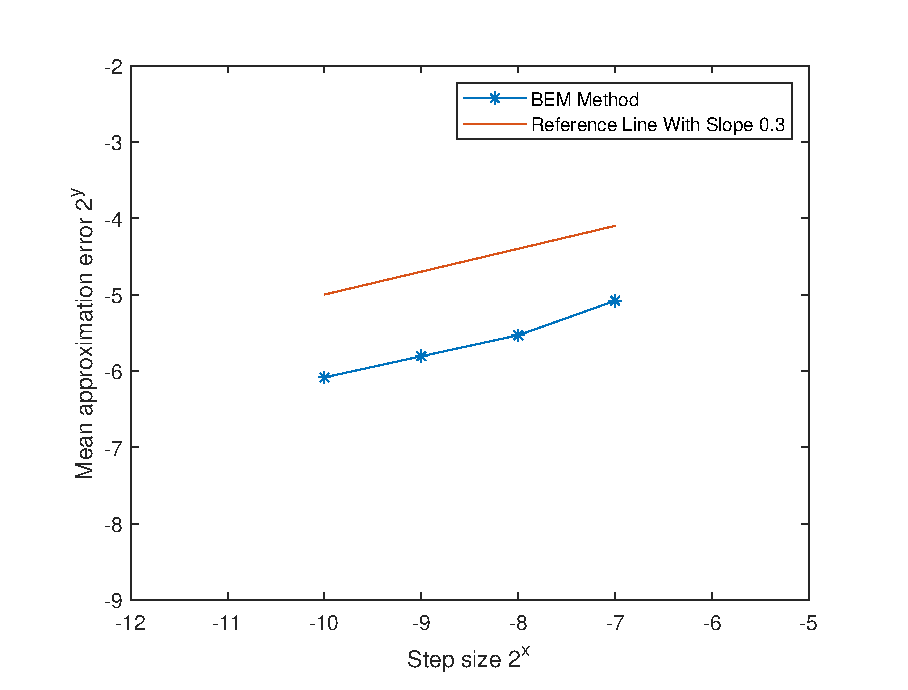
\includegraphics[width=0.45\linewidth]{BEMalpha=0.3.eps}
	\hfill
	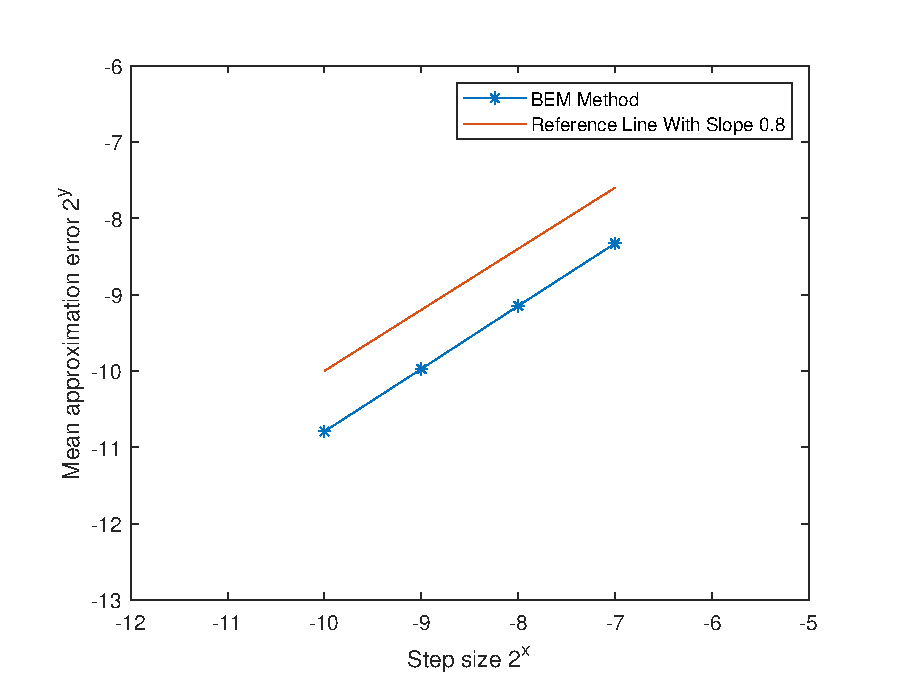
\includegraphics[width=0.45\linewidth]{BEMalpha=0.8.eps}
	\caption{时间变换CIR过程的数值解与解析解之间的绝对误差估计.左图是$\alpha=0.3$,右图是$\alpha=0.8$}
	\label{fig:image}
	\vspace{-2ex}
\end{figure}

%	\section{Present Job}
%	我们想证明的是对于一个漂移项和扩散项都是非线性的时间变换SDE,将它进行Lamperti变换,变成漂移项是非线性,扩散项是常数的时间变换SDE,然后使用数值方法进行离散,得到与模拟代码一致的强收敛阶$\alpha$.截止当前的证明,我们已经证明了显式EM在$L^1$误差下的强收敛阶是$\alpha$,在证明$L^p$时,若使用之前的方法,得到的强收敛阶不仅与模拟的结果不一致,并且与p有关,强收敛阶与模拟代码不一致.证明的显示EM的强收敛阶,看起来对我们的预期没有什么意义,至少暂时我还没有找到对于原始非线性的漂移项扩散项经过Lamperti变换之后,得到的时变SDE漂移项满足全局Lipschitz,进而能够使用显示EM得到强收敛阶.下面对于变换后非线性的SDE,采用截断EM或者BEM,都会出现一个难以处理的东西,我们必须计算$L^2$误差,也就是$e^2$,这将导致不得不使用Gronwall不等式来处理这个式子,此时也会出现完全与p相关的收敛阶,那么我们可能需要换一个方法了.
%	由于无法处理$L^2$误差,因此对于单调Lipschitz条件出现的平方项就无法使用.
%	\textcolor{red}{至于Gronwall不等式,他在积分方面是几乎无法使用的,如果你选择先期望再Gronwall,会发现期望无法进入积分里面,这就导致了Gronwall条件不成立.然而如果先Gronwall再期望,则会发现离Gronwall条件相差十万八千里}